
% Source: paper/sections/*-en.md + paper/tables/*-en.md (committed 13b8889).
% Numbers verified against the Norwegian canonical: T = 0.0922, K = 0.004986,
% T/sigma_diff = 2.73 / 1.80, M = 2/5, M' = 3/5, etc.
% Figures in paper/arxiv/figures/*.pdf (vector, generated from
% paper/plot_methods_figures.py with dejargonized English captions).

\documentclass[11pt,a4paper]{article}

\usepackage[utf8]{inputenc}
\usepackage[T1]{fontenc}
\usepackage{lmodern}
\usepackage{microtype}
\usepackage[margin=1in]{geometry}
\usepackage{amsmath,amssymb}
\usepackage{graphicx}
\usepackage{booktabs}
\usepackage{array}
\usepackage{hyperref}
\usepackage{xcolor}
\usepackage{natbib}
\usepackage{caption}
\usepackage{titlesec}

\hypersetup{
  colorlinks=true,
  linkcolor=blue!50!black,
  citecolor=blue!50!black,
  urlcolor=blue!50!black
}

% Tighter section spacing
\titlespacing*{\section}{0pt}{1.5ex plus 1ex minus .2ex}{1ex plus .2ex}
\titlespacing*{\subsection}{0pt}{1.2ex plus 1ex minus .2ex}{0.8ex plus .2ex}

% Code identifiers
\newcommand{\code}[1]{\texttt{#1}}

\title{A Criterion-Validity Gate for Threshold-Based Reproducibility Assessment in RL}

\author{
% PLACEHOLDER --- Eirik to confirm affiliation, email, ORCID.
Eirik Botten Nicolaysen\\
EcoDeco AS\\
\texttt{[email pending]}
}

\date{\today}

\begin{document}
\maketitle

\begin{abstract}
RL agents are evaluated against thresholds that are rarely validated against the noise inside their own measurement window. A threshold can be meaningful against the outcome span and at the same time noise-dominated in the window where it is actually applied --- and when that happens, an apparently clean result is a measurement artefact. Which seeds pass is closer to a coin flip than to a finding.

We pre-registered an evaluation of an RL agent against an ethological simulator in an ACI (animal-computer interaction) context, and introduced a \emph{criterion-validity gate}: a check, registered together with the methodology, that verifies the threshold is separable from the noise in its application window before it is applied. The gate changed the outcome in three documented cases. A climb-leg was being measured against a window where the noise sat at roughly $10\times$ the threshold --- an inconsistency we had built in ourselves. The measurement window turned out to be direction-symmetric: it hid the observed phenomenon on some seeds and fabricated it on others. And on escalation, the gate failed on a fresh seed batch because the noise scale was roughly $50\%$ higher under identical configuration.

The last result is the point. The phenomenon could not be decided as robust or not-robust on attainable compute --- not for lack of data, but because measurability itself is seed-variable, at a level deeper than the phenomenon. The contribution is the method that made that refusal pre-registered and visible instead of producing a false clean number. Wherever a reproducibility threshold risks sitting inside the noise of the window it is applied to --- a common case in RL evaluation --- gate-protected pre-registration is the infrastructure that lets pre-registration deliver what it promises: honest assessment instead of clean-looking artefacts.
\end{abstract}

\section{Introduction}

\subsection{}
\label{sec:1.1}

Reproducibility assessment for reinforcement-learning agents rests on thresholds: a metric crosses a line and a run is called clean, or it does not and the run is flagged. The line is the whole judgment. But a threshold can look principled and still be noise-dominated inside the window it is applied to --- and when that happens, a result that reads as clean is a measurement artifact, not a finding. Pre-registration does not catch this on its own. Fixing the threshold and the analysis in advance guards against the obvious failure --- choosing a cutoff after seeing the data --- but it says nothing about whether the chosen cutoff sits above or below the noise floor of the very quantity it gates. A pre-registered threshold that lands inside the noise band is still a clean-looking artifact. It is just an honestly arrived-at one.

We demonstrate the method on an RL agent trained against an ethological simulator --- chatcat, a companion-AI substrate for animal behavior. The domain is not incidental, and it is not the subject of the paper. We name it because its documented failure mode is overclaiming, which makes it a high-stakes test case: here, a false clean result costs something. The reference point is MeowTalk. \citet{ntalampiras2019} established, as a proof of concept, that the emission context of a meow can be classified into three contexts --- narrow, falsifiable science, and it holds. The product built on top of it stretched that foundation into translation claims it could not support --- a gap one of the app's own creators later conceded to the New York Times \citep{anthes2022}. The distance between what the science carried and what the product asserted is the failure mode, and a field that fails this way is exactly where an evaluation that refuses to overclaim earns its keep. Companion-AI for animals is not what the paper is about; it is the sharpest place to show a method that does not fool itself.

The simulator itself is seriously constructed, not a toy dressed up for the argument. Its design is litterbox-first and uses no live animal, following the animal-computer-interaction lineage --- the Cat Royale work \citep{schneiders2024} and the ethical position set out by \citet{vanpatter2020} and \citet{mancini2023}, where non-maleficence and voluntary participation are treated as design constraints rather than disclaimers. That lineage is why the substrate is the kind of thing a method can be tested against at all. But the substrate is the test bench, not the contribution. What this paper offers is an evaluation method --- a criterion-validity gate --- that stopped us from reporting a clean result we had not in fact earned, and that generalizes to any threshold-based reproducibility assessment in RL. Section~\ref{sec:1.2} sets out the gap --- a threshold validated against outcome-spread rather than window-noise --- and Section~\ref{sec:1.3}, the gate that closes it.

\subsection{}
\label{sec:1.2}

RL evaluation rarely pre-registers. When it does, the threshold is registered, but not whether the threshold is separable from the noise in the window it is measured against. That is the gap.

A threshold $T$ can be validated against the outcome span --- peak to end --- and look meaningful. The same $T$ can be noise-dominated in the window where $T$ is actually applied --- \code{ep\_init}, the mean of returns over a defined early-training window. When it is, whether a given seed passes is close to a coin flip. The result reads as a finding about the agent; it is a finding about the window.

\subsection{}
\label{sec:1.3}

Our contribution is a criterion-validity gate: a pre-registered check, run before the threshold is applied, that $T$ is separable from the noise-difference in its application window. Operationally we require that $T$ sit at least roughly twice above the noise-difference in the window. The gate is registered together with the methodology, not added afterwards.

We report three cases in which the gate changed the outcome. None are hypothetical --- each is measured, and each points to a committed assumption in an ADR chain that forms the paper's reproducible appendix. The negative outcome is the contribution: that we could not decide the phenomenon, together with the precise reason no reasonable amount of compute would have changed that, is a stronger methodological result than a number we would have had to force.

\subsection{}
\label{sec:1.4}

The paper delimits what it claims. It does not claim that the phenomenon we observed --- climb-then-slide, where the agent reaches baseline and does not hold it --- is solved. It claims no fix; warm-start, KL-anchoring, and reward-reshaping are all unchosen and lie downstream. It does not claim the simulator is realistic; the sim-to-real gap is undocumented until v0.4, and we note this explicitly. The diagnosis we made --- that the slide sits on the optimisation side, not in the reward landscape --- is diagnosis, not fix, and is presented as such.

\subsection{}




\section{Methods}

\subsection{Setup}
\label{sec:2.1}

We trained an RL agent against an ethological simulator (SimCat) in a companion-AI context. The agent is CleanRL's \code{ppo\_continuous\_action} over a continuous action space $\mathrm{Box}(7,)$, with a stdio bridge between the Python side running RL and the TypeScript runtime running the simulator. Reward is baseline-normalised: $R_\mathrm{agent} - R_\mathrm{baseline}$. This is the setup in which the phenomenon we study arises --- climb-then-slide, where the agent climbs to the baseline line and does not hold it.

Each run is about 5M steps, roughly 33 minutes CPU. Runs are deterministic per seed; we verified this by an interrupted run overlapping bit-identically with its restart over 1391 updates. Artefacts live on persistent storage, not on a volatile path --- a point we return to, because an earlier dataset was lost and forced reconstruction.

\subsection{Pre-registration discipline}
\label{sec:2.2}

Every methodological decision was locked and pushed to version control before data was collected or training was run. Metrics, thresholds, success criteria, and falsification conditions are committed in advance. Pre-registration is not novel in principle --- what we do is apply it with a precision RL evaluation rarely has: the full decision trail lives chronologically in the version history, and every claim in the results points to the commit that locked the assumption it rests on. The pattern repeated over four iterations through the work.

\subsection{Anchoring seed}
\label{sec:2.3}

The thresholds are measured, not guessed. Two thresholds govern the evaluation: $T$ for climb/slide, $K$ for critic-convergence. Both are anchored in measured scale from one dedicated anchoring run rather than in a chosen number. The anchoring seed measures the scale quantities --- inter-update SD over a defined window (after the rolling 100-episode buffer has filled), median \code{value\_loss} over a late window --- and $T$ and $K$ are set as multiples of these.

One discipline here is decisive. The anchoring seed's own outcome --- whether it itself reproduced the phenomenon --- is never read and does not count as a data point. It sets scale, not result. If we let it count as both, the criterion would become circular: a seed that helped define the threshold could not at the same time be an independent test of it.

The numbers: $T = 0.0922$, three times the late-stable inter-update SD of $0.0307$. $K = 0.004986$, three times the median \code{value\_loss} of $0.001662$. The multipliers were locked before measurement and justified noise-statistically --- roughly two standard deviations outside the noise-difference --- not tuned to hit a desired outcome.

\subsection{Criterion-validity gate}
\label{sec:2.4}

This is the contribution. Before a threshold is applied, we verify that it is separable from the noise in its own application window: $T$ must sit at least roughly twice above the noise-difference in that window. We write $\sigma_\mathrm{diff} = \sigma \times \sqrt{2}$ for the noise in the difference between two window means (under a simplifying independence assumption).

Why it is needed: standard pre-registration locks the threshold and validates it against the outcome span, peak minus end. It does not validate it against the noise in the window the threshold is actually measured against. A threshold can pass the first check and still be noise-dominated in the application window. When it is, which seeds pass is close to random --- and the result reads as a finding about the agent when it is a finding about the window.

The gate has a pre-registered binary outcome. PASS: the threshold is valid, the evaluation proceeds. FAIL: the threshold is noise-dominated in this window, and we stop instead of applying it. We ran the gate twice. It passed the first time ($T/\sigma_\mathrm{diff} = 2.73$) and failed the second ($T/\sigma_\mathrm{diff} = 1.80$). That it failed on a real dataset (the N=15 escalation, $T/\sigma_\mathrm{diff} = 1.80$) shows that the PASS in the criterion-validity reanalysis ($T/\sigma_\mathrm{diff} = 2.73$) was not predetermined by construction.

\subsection{Falsification structure}
\label{sec:2.5}

The success criterion and the falsification were pre-registered: how many seeds must reproduce the phenomenon for it to count as robust, and what counts as not-robust. The escalation added a third outcome that is the most important design choice in the whole structure. The middle band (the middle outcome band, pre-registered as ``intrinsically seed-variable'') is a real finding, not a failed test. If the phenomenon occurs about half the time without hidden structure beneath it, \emph{that} is the answer --- the phenomenon is intrinsically seed-variable --- and not a call for more compute. We pre-registered that outcome precisely to close the infinite-escalation trap: without a defined middle band, an ambiguous result can always justify one more run, indefinitely.

To distinguish an optimisation artefact from a feature of the reward landscape, we pre-registered a diagnostic signature, SIG-EXPLORATION: if the variance in the policy (\code{actor\_logstd\_mean}) does not collapse while the critic (\code{value\_loss}) converges low, the slide sits on the optimisation side. The signature is read from logs that already exist --- it costs no new training.

\subsection{Reproducibility}
\label{sec:2.6}

The entire decision-and-evidence trail lives as an ADR chain in the version history, chronological, stub before resolution. Every threshold, every gate, every outcome points to a commit hash. All the runs the paper builds on come from one seed set under identical configuration, and the figures and tables are traceable to the same dataset --- not to an earlier set that was lost. The ADR chain is the reproducible appendix; the plotting scripts sit next to the figures they generate.

\section{Results}

\subsection{The phenomenon in form}
\label{sec:3.1}

All five seeds in $\{6 \ldots 10\}$ climb to a peak and slide back. In form, climb-then-slide is universal --- $5/5$ --- and this is what the curves show directly (Fig.~\ref{fig:1}). But form is not the same as amplitude against a threshold. Whether the climb leg actually passes $T$ depends on which window we measure it in, and that distinction --- form versus amplitude-against-threshold --- is the whole point of what follows.

\begin{figure}[h]
\centering
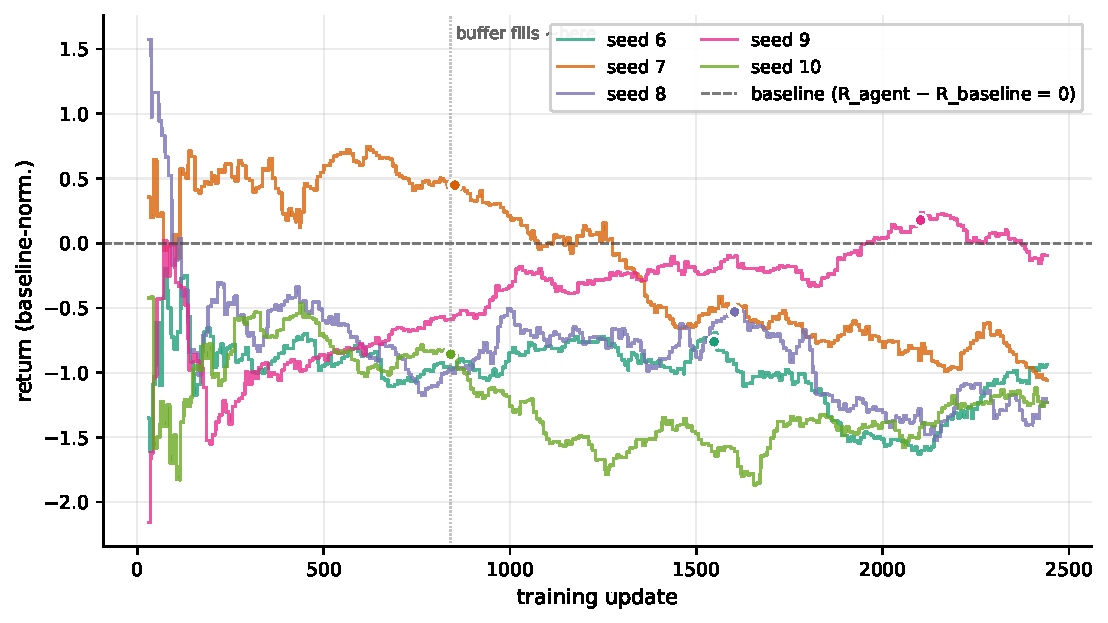
\includegraphics[width=0.95\linewidth]{figures/fig1_climb_then_slide.pdf}
\caption{Climb-then-slide in FORM on N=5 seeds $\{6 \ldots 10\}$. All five seeds climb to a peak and slide back (climb-then-slide in FORM = 5/5; slide-direction confirmed universal across all five seeds). Dots mark each seed's peak update. Whether the amplitude passes $T = 0.0922$ for the climb-leg depends on the \code{ep\_init} measurement window --- that distinction is the subject of Fig.~\ref{fig:3}.}
\label{fig:1}
\end{figure}

\subsection{The direction-symmetric confounder}
\label{sec:3.2}

We write CTS (climb-then-slide) when we refer to whether a seed reproduced the phenomenon against the threshold, and $M$, $M'$, $M''$ for the reproduction count in each of the three measurement passes. The same measurement window lied both ways (Fig.~\ref{fig:3}). With the original \code{ep\_init} window $[100, 150]$, seeds 6 and 8 measured their climb leg below $T$ --- not reproduced. Moved to the buffer-full window, the same two passed above $T$. The window had hidden real climb-then-slide. At the same time seed 10 went the other way: above $T$ in the original window, below $T$ in the revised one. The window had fabricated a phenomenon that was not there.

That is the key finding. A window change that had only hidden, or only fabricated, could be dismissed as a one-way bias one corrects for. That the same change moved two seeds into a positive result and a third out of it, simultaneously, shows that which seeds pass is governed by the measurement choice, not by the agent. The numbers shifted accordingly: $M$ against the original window was $2/5$, $M'$ against the buffer-full one was $3/5$ (Table~\ref{tab:2}).

\begin{figure}[h]
\centering
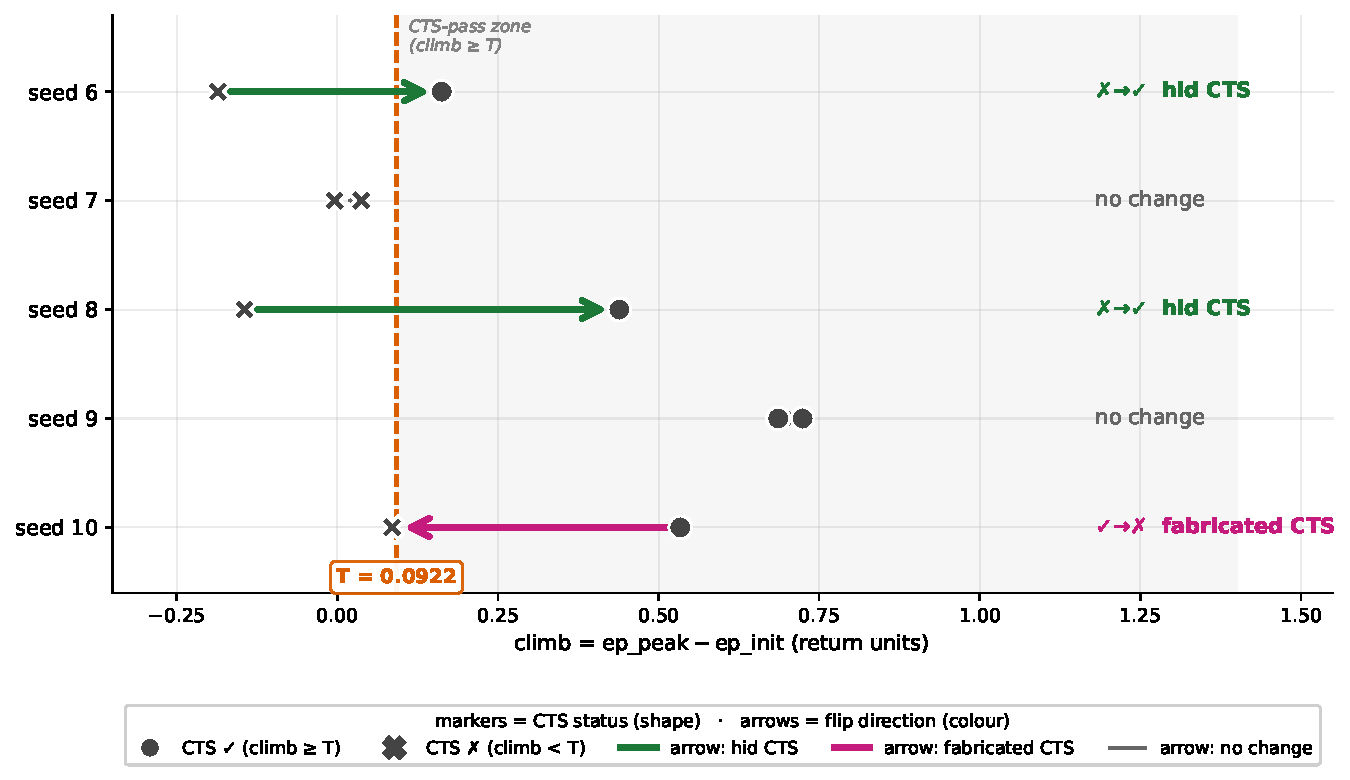
\includegraphics[width=0.95\linewidth]{figures/fig3_confounder_symmetric.pdf}
\caption{Direction-symmetric \code{ep\_init}-window confounder on seeds $\{6 \ldots 10\}$ (KEY). Each arrow shows one seed's climb shifting between \code{ep\_init} windows: tail = original $[100, 150]$ window; head = revised buffer-full window. The confounder lied both ways: seeds 6 and 8 had real CTS hidden by buffer noise (green, $\times \to \checkmark$); seed 10's apparent CTS was a buffer-noise artefact (magenta, $\checkmark \to \times$). $M: 2/5 \to M': 3/5$. Marker colours are neutral by design --- the colour story here is flip direction (arrows). Fig.~\ref{fig:1}'s per-seed colours code seed identity, a separate scheme.}
\label{fig:3}
\end{figure}

\begin{table}[h]
\centering
\caption{Phenomenon-reproduction count across measurement passes. Climb-then-slide reproduction count $M / M' / M''$ across the three measurement passes on the same phenomenon-question. $T = 0.0922$ (locked from the original pre-registration); the only thing that changes is the \code{ep\_init} window definition.}
\label{tab:2}
\small
\begin{tabular}{@{}llllllr l@{}}
\toprule
Pass & Measurement pass & Seeds & \code{ep\_init} window & Gate & Count & Reading \\
\midrule
$M$    & original pre-registration   & $\{6 \ldots 10\}$       & original $[100,150]$ & not built yet                                    & $\mathbf{2/5}$ & robustness falsification triggers on locked criterion \\
$M'$   & criterion-validity reanalysis & $\{6 \ldots 10\}$     & revised buffer-full  & PASS ($T/\sigma_\mathrm{diff}\!=\!2.73$)         & $\mathbf{3/5}$ & borderline, inconclusive on N=5 reanalysis budget \\
$M''$  & N=15 escalation             & $\{11 \ldots 20\}$ added & revised buffer-full & \textbf{FAIL ($T/\sigma_\mathrm{diff}\!=\!1.80$)} & not tallied   & climb readout not performed per the pre-registered gate \\
\bottomrule
\end{tabular}

\vspace{1em}

\textit{Per-seed flips between $M$ and $M'$ (same data, only \code{ep\_init} window changed):}

\vspace{0.5em}

\begin{tabular}{@{}rrrcc l@{}}
\toprule
Seed & climb ($M$, $[100,150]$) & climb ($M'$, revised) & CTS $M$ & CTS $M'$ & Flip \\
\midrule
6  & $-0.1860$ & $+0.1624$ & $\times$ & $\checkmark$ & $\times \to \checkmark$ (confounder hid CTS) \\
7  & $+0.0373$ & $-0.0040$ & $\times$ & $\times$ & no change \\
8  & $-0.1445$ & $+0.4391$ & $\times$ & $\checkmark$ & $\times \to \checkmark$ (confounder hid CTS) \\
9  & $+0.6863$ & $+0.7242$ & $\checkmark$ & $\checkmark$ & no change \\
10 & $+0.5340$ & $+0.0852$ & $\checkmark$ & $\times$ & $\checkmark \to \times$ (confounder fabricated CTS) \\
\bottomrule
\end{tabular}
\end{table}

\subsection{The mechanism}
\label{sec:3.3}

On the seeds that reproduce climb-then-slide, the SIG-EXPLORATION signature holds (Fig.~\ref{fig:2}). The variance in the policy does not collapse during peak, and the critic is converged low. The slide is the optimisation side of a wide-variance policy, not a result of variance collapse. The pattern is the same on all reproducing seeds, across both measurement passes.

\begin{figure}[h]
\centering
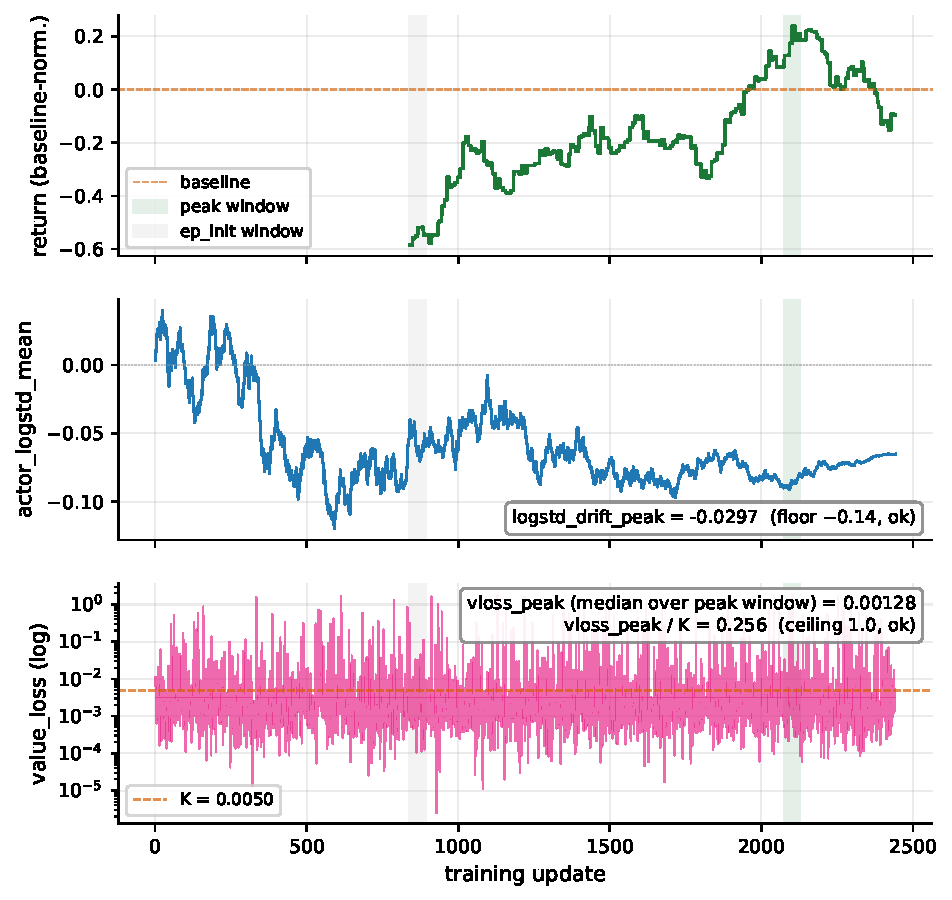
\includegraphics[width=0.95\linewidth]{figures/fig2_sig_exploration.pdf}
\caption{SIG-EXPLORATION signature on seed 9 (CTS-reproducing in both measurement passes). Top panel shows the same \code{ep\_return\_mean\_recent} series as Fig.~\ref{fig:1}, zoomed in on the buffer-full eligible region (update $\geq 841$); y-axis values are identical where the x-axes overlap (e.g., seed 9 peak $= 0.2379$ at update 2102 in both figures). Variance (\code{actor\_logstd}) does not collapse during peak; critic (\code{value\_loss}) is converged low. The mechanism (SIG-EXPLORATION) holds: slide is the optimisation side of a wide-variance policy, not variance-collapse. Same pattern on all CTS-reproducing seeds across both passes.}
\label{fig:2}
\end{figure}

\subsection{The gate passed, then failed}
\label{sec:3.4}

In the criterion-validity reanalysis the gate passed --- $T/\sigma_\mathrm{diff} = 2.73$ --- and $M'$ landed at $3/5$. Borderline, and inconclusive on five seeds. The N=15 escalation added ten new seeds, $\{11 \ldots 20\}$, for N=15. There the gate failed: $T/\sigma_\mathrm{diff} = 1.80$. The same training configuration produced a median noise scale roughly $50\%$ higher on the new seed set, $0.0362$ against $0.0239$ (Fig.~\ref{fig:4}, Table~\ref{tab:1}). The stop rule was triggered before $M''$ was tallied.

The finding sits there. Measurability itself is seed-variable: the noise scale $T$ was anchored against on one seed set does not hold on another under identical configuration. That is one level deeper than the phenomenon. We cannot decide whether climb-then-slide is robust --- not because we lack data, but because the threshold is not stably applicable across seeds.

\begin{figure}[h]
\centering
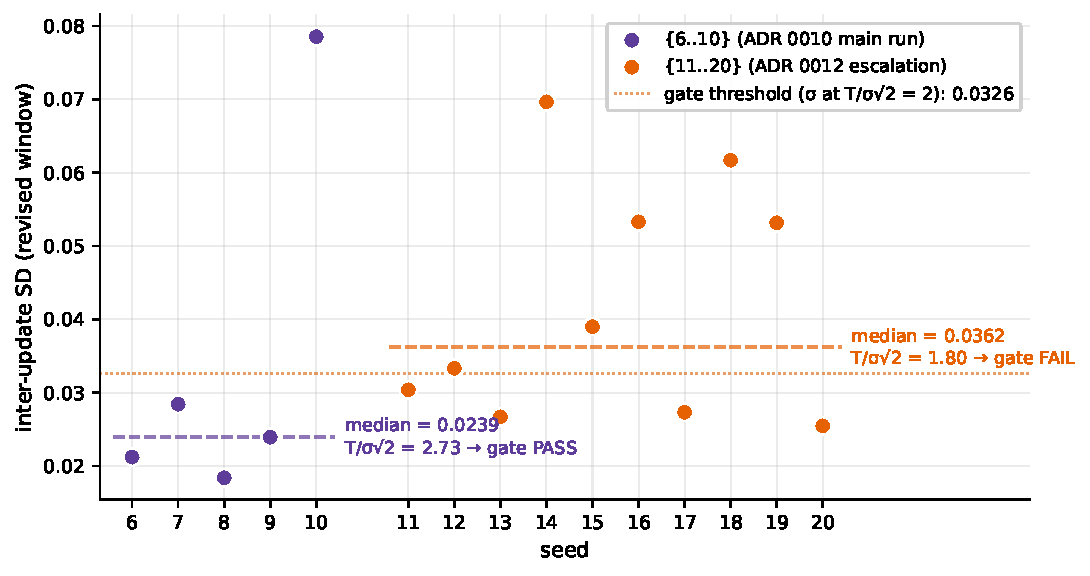
\includegraphics[width=0.95\linewidth]{figures/fig4_noise_scale_comparison.pdf}
\caption{Same training config, $\sim 50\%$ different median noise scale across seed-batches. Per-seed inter-update SD of \code{ep\_return\_mean\_recent} in each seed's revised buffer-full \code{ep\_init} window. Identical training config produces medians $0.024$ vs $0.036$ ($50\%$ difference) across the two seed-batches --- large enough to flip the criterion-validity gate from PASS ($2.73$) to FAIL ($1.80$) without any methodology change.}
\label{fig:4}
\end{figure}

\begin{table}[h]
\centering
\caption{Criterion-validity gate: criterion-validity reanalysis PASS vs N=15 escalation FAIL. Per-seed inter-update SD of \code{ep\_return\_mean\_recent} over each seed's revised buffer-full \code{ep\_init} window (first 51 updates with \code{ep\_return\_n\_recent} $\geq 100$). Gate fires if $T / (\sigma_\mathrm{median} \times \sqrt{2}) \geq \sim 2$.}
\label{tab:1}
\small
\begin{tabular}{@{}rrl@{}}
\toprule
Seed & Inter-update SD & Group \\
\midrule
6  & $0.021220$ & $\{6 \ldots 10\}$ (criterion-validity reanalysis) \\
7  & $0.028428$ & $\{6 \ldots 10\}$ (criterion-validity reanalysis) \\
8  & $0.018406$ & $\{6 \ldots 10\}$ (criterion-validity reanalysis) \\
9  & $0.023918$ & $\{6 \ldots 10\}$ (criterion-validity reanalysis) \\
10 & $0.078524$ & $\{6 \ldots 10\}$ (criterion-validity reanalysis) \\
11 & $0.030381$ & $\{11 \ldots 20\}$ (N=15 escalation) \\
12 & $0.033319$ & $\{11 \ldots 20\}$ (N=15 escalation) \\
13 & $0.026707$ & $\{11 \ldots 20\}$ (N=15 escalation) \\
14 & $0.069636$ & $\{11 \ldots 20\}$ (N=15 escalation) \\
15 & $0.039013$ & $\{11 \ldots 20\}$ (N=15 escalation) \\
16 & $0.053293$ & $\{11 \ldots 20\}$ (N=15 escalation) \\
17 & $0.027316$ & $\{11 \ldots 20\}$ (N=15 escalation) \\
18 & $0.061690$ & $\{11 \ldots 20\}$ (N=15 escalation) \\
19 & $0.053154$ & $\{11 \ldots 20\}$ (N=15 escalation) \\
20 & $0.025466$ & $\{11 \ldots 20\}$ (N=15 escalation) \\
\bottomrule
\end{tabular}

\vspace{1em}

\textit{Aggregate (per group):}

\vspace{0.5em}

\begin{tabular}{@{}lrr@{}}
\toprule
                                    & $\{6 \ldots 10\}$ (criterion-validity reanalysis) & $\{11 \ldots 20\}$ (N=15 escalation) \\
\midrule
n seeds                             & 5             & 10            \\
median $\sigma$                     & $\mathbf{0.023918}$ & $\mathbf{0.036166}$ \\
$\sigma_\mathrm{diff} = \sigma \times \sqrt{2}$ & $0.033826$    & $0.051146$    \\
$T / \sigma_\mathrm{diff}$          & $\mathbf{2.7257}$   & $\mathbf{1.8027}$   \\
Gate decision (threshold $\geq \sim 2$) & \textbf{PASS} & \textbf{FAIL} \\
\bottomrule
\end{tabular}

\vspace{0.5em}

\small $T = 0.0922$ (locked since commit \code{0140536}). The gate was triggered in opposite directions on the two batches despite identical training configuration --- evidence that the gate is not a formality and that same-config noise scale is itself substantial.
\end{table}

\section{Discussion}

\subsection{What the result actually is}
\label{sec:4.1}

The outcome is negative and inconclusive, but it is not empty. We did not decide the phenomenon. We decided that the phenomenon cannot be decided with this threshold approach on attainable compute, and we know precisely why: measurability is seed-variable. That is the difference between ``we do not know'' and ``we know why we cannot know with this method.'' The second is a result.

\subsection{Why the gate is the contribution}
\label{sec:4.2}

Without the gate, the criterion-validity reanalysis's $M' = 3/5$ would have been reported as a borderline finding about the agent, and the N=15 escalation's new seeds would have produced an $M''$ figure that looked like data. The gate showed that both would in fact have been findings about the measurement window, not the agent, and refused to produce a clean number where the number would have been an artefact. Within RL evaluation, this generalises this far and no further: any threshold-based reproducibility assessment where the threshold is anchored in one regime and applied in another is vulnerable to this failure, and the gate is a cheap check against it. It is a check against one failure class, not a solution to RL evaluation.

\subsection{Limitations}
\label{sec:4.3}

The simulator is not realistic; the sim-to-real gap is undocumented until v0.4. The results apply to agent evaluation in simulator, not cat behaviour, and we claim nothing else. N=15 is small --- but that is precisely the point. More N does not solve the problem when measurability itself is seed-variable, and that is why the middle band was pre-registered as an endpoint rather than a place to draw more runs from. The diagnosis is diagnosis, not fix: we point out that the slide is on the optimisation side, we do not solve it. Warm-start, KL-anchoring, and reward-reshaping are all unchosen and lie downstream.


\label{sec:4.4}





\subsection{Closing}


What we offer the field is not an answer to climb-then-slide. It is a method that refused to give a false answer, and an explicit trail of why that refusal was the right scientific action. In a field where overclaiming is the documented failure mode, evaluation infrastructure that can say ``this cannot be decided yet, and here is why'' is a precondition for not becoming what one criticises.

\bibliographystyle{plainnat}
\bibliography{refs}

\appendix

\section{The ADR chain as a reproducible evidence trail}
\label{app:A}

The entire decision-and-evidence trail for the evaluation lives committed on the project's \code{origin/main}. Every claim in Section~\ref{sec:1.3}--Section~\ref{sec:3.4} (results, anchoring seed, gate, falsification structure) points to one of these commits as the lock for the assumption it rests on. Stub commits locked the methodology before data; resolution commits reported the outcome against the already-frozen methodology. ADR numbers are retained in this appendix as a cross-reference index; the main text above uses semantic descriptions (``the original pre-registration'', ``the criterion-validity reanalysis'', ``the N=15 escalation'').

\begin{table}[h]
\centering
\small
\begin{tabular}{@{}p{0.32\linewidth}lp{0.10\linewidth}p{0.40\linewidth}@{}}
\toprule
Phase & Commit & Date & What was locked / reported \\
\midrule
\multicolumn{4}{l}{\textbf{ADR 0010 --- original criterion}} \\
Stub (framing question + SIG-EXPLORATION diagnosis) & \code{31c363e} & 2026-06-03 & Structural-finding framing chosen (not a deployable fix); mechanism diagnosis on partial data from the prior evaluation round \\
Pre-reg ($T$ and $K$ locked from anchoring seed)    & \code{0140536} & 2026-06-04 & $T = 0.0922$, $K = 0.004986$, peak window, falsifiers F1--F4 \\
Resolution (main run $\{6 \ldots 10\}$, F3 triggered) & \code{1ba60c0} & 2026-06-05 & $M = 2/5$ against locked criterion; climb-window confounder documented \\
\multicolumn{4}{l}{\textbf{ADR 0011 --- criterion-validity gate introduced}} \\
Stub (gate pre-registered)                          & \code{4647ed8} & 2026-06-05 & Revised \code{ep\_init} window, gate formula, three-way $M'$ outcome \\
Resolution (reanalysis, gate PASS, $M' = 3/5$)      & \code{8e977f1} & 2026-06-05 & $T/\sigma_\mathrm{diff} = 2.7257$ PASS; three seeds flipped CTS status \\
\multicolumn{4}{l}{\textbf{ADR 0012 --- escalation to N=15}} \\
Stub (N=15 + three-way success + middle-band discipline) & \code{3e45ac7} & 2026-06-05 & Seeds $\{11 \ldots 20\}$, middle band as endpoint \\
Resolution (gate FAIL, $M''$ not tallied)           & \code{7e4dbd9} & 2026-06-06 & $T/\sigma_\mathrm{diff} = 1.8027$ FAIL; $\sim 50\%$ noise-scale discrepancy \\
\multicolumn{4}{l}{\textbf{Supporting commits}} \\
Instrumentation (\code{actor\_logstd} logging + checkpoint-on-best) & \code{cd5def3} & 2026-06-04 & \code{metrics.jsonl} schema extended for SIG-EXPLORATION reading \\
Figures + plotting script                           & \code{e05300b} & 2026-06-06 & Fig.~1--4 + Table~1--2 reproducible from \code{metrics.jsonl} \\
Source-attribution correction (4 verified refs)     & \code{62bccf8} & 2026-06-06 & The four Section~\ref{sec:1.1} citations locked against verified originals \\
\bottomrule
\end{tabular}
\end{table}

\subsection*{Reproducibility}

All training runs live as \code{metrics.jsonl} + \code{agent.pt} + \code{best\_so\_far.pt} under \code{\textasciitilde/chatcat-rl-runs/} (persistent path, documented in ADR 0010 Step 1.5). The plotting script \code{paper/plot\_methods\_figures.py} regenerates Fig.~1--4 and Tables~1--2 from the same \code{metrics.jsonl} files; no new training is required to reproduce the figures. Vector export (PDF) for submission is produced by the same script.

\end{document}
